\PassOptionsToPackage{unicode=true}{hyperref} % options for packages loaded elsewhere
\PassOptionsToPackage{hyphens}{url}
%
\documentclass[ignorenonframetext,]{beamer}
\usepackage{pgfpages}
\setbeamertemplate{caption}[numbered]
\setbeamertemplate{caption label separator}{: }
\setbeamercolor{caption name}{fg=normal text.fg}
\beamertemplatenavigationsymbolsempty
% Prevent slide breaks in the middle of a paragraph:
\widowpenalties 1 10000
\raggedbottom
\setbeamertemplate{part page}{
\centering
\begin{beamercolorbox}[sep=16pt,center]{part title}
  \usebeamerfont{part title}\insertpart\par
\end{beamercolorbox}
}
\setbeamertemplate{section page}{
\centering
\begin{beamercolorbox}[sep=12pt,center]{part title}
  \usebeamerfont{section title}\insertsection\par
\end{beamercolorbox}
}
\setbeamertemplate{subsection page}{
\centering
\begin{beamercolorbox}[sep=8pt,center]{part title}
  \usebeamerfont{subsection title}\insertsubsection\par
\end{beamercolorbox}
}
\AtBeginPart{
  \frame{\partpage}
}
\AtBeginSection{
  \ifbibliography
  \else
    \frame{\sectionpage}
  \fi
}
\AtBeginSubsection{
  \frame{\subsectionpage}
}
\usepackage{lmodern}
\usepackage{amssymb,amsmath}
\usepackage{ifxetex,ifluatex}
\usepackage{fixltx2e} % provides \textsubscript
\ifnum 0\ifxetex 1\fi\ifluatex 1\fi=0 % if pdftex
  \usepackage[T1]{fontenc}
  \usepackage[utf8]{inputenc}
  \usepackage{textcomp} % provides euro and other symbols
\else % if luatex or xelatex
  \usepackage{unicode-math}
  \defaultfontfeatures{Ligatures=TeX,Scale=MatchLowercase}
\fi
\usetheme[]{Boadilla}
\usecolortheme{seahorse}
% use upquote if available, for straight quotes in verbatim environments
\IfFileExists{upquote.sty}{\usepackage{upquote}}{}
% use microtype if available
\IfFileExists{microtype.sty}{%
\usepackage[]{microtype}
\UseMicrotypeSet[protrusion]{basicmath} % disable protrusion for tt fonts
}{}
\IfFileExists{parskip.sty}{%
\usepackage{parskip}
}{% else
\setlength{\parindent}{0pt}
\setlength{\parskip}{6pt plus 2pt minus 1pt}
}
\usepackage{hyperref}
\hypersetup{
            pdftitle={An Application of Principal Components Analysis in Genetics},
            pdfauthor={Sam Morrissette},
            pdfborder={0 0 0},
            breaklinks=true}
\urlstyle{same}  % don't use monospace font for urls
\newif\ifbibliography
\usepackage{color}
\usepackage{fancyvrb}
\newcommand{\VerbBar}{|}
\newcommand{\VERB}{\Verb[commandchars=\\\{\}]}
\DefineVerbatimEnvironment{Highlighting}{Verbatim}{commandchars=\\\{\}}
% Add ',fontsize=\small' for more characters per line
\usepackage{framed}
\definecolor{shadecolor}{RGB}{248,248,248}
\newenvironment{Shaded}{\begin{snugshade}}{\end{snugshade}}
\newcommand{\AlertTok}[1]{\textcolor[rgb]{0.94,0.16,0.16}{#1}}
\newcommand{\AnnotationTok}[1]{\textcolor[rgb]{0.56,0.35,0.01}{\textbf{\textit{#1}}}}
\newcommand{\AttributeTok}[1]{\textcolor[rgb]{0.77,0.63,0.00}{#1}}
\newcommand{\BaseNTok}[1]{\textcolor[rgb]{0.00,0.00,0.81}{#1}}
\newcommand{\BuiltInTok}[1]{#1}
\newcommand{\CharTok}[1]{\textcolor[rgb]{0.31,0.60,0.02}{#1}}
\newcommand{\CommentTok}[1]{\textcolor[rgb]{0.56,0.35,0.01}{\textit{#1}}}
\newcommand{\CommentVarTok}[1]{\textcolor[rgb]{0.56,0.35,0.01}{\textbf{\textit{#1}}}}
\newcommand{\ConstantTok}[1]{\textcolor[rgb]{0.00,0.00,0.00}{#1}}
\newcommand{\ControlFlowTok}[1]{\textcolor[rgb]{0.13,0.29,0.53}{\textbf{#1}}}
\newcommand{\DataTypeTok}[1]{\textcolor[rgb]{0.13,0.29,0.53}{#1}}
\newcommand{\DecValTok}[1]{\textcolor[rgb]{0.00,0.00,0.81}{#1}}
\newcommand{\DocumentationTok}[1]{\textcolor[rgb]{0.56,0.35,0.01}{\textbf{\textit{#1}}}}
\newcommand{\ErrorTok}[1]{\textcolor[rgb]{0.64,0.00,0.00}{\textbf{#1}}}
\newcommand{\ExtensionTok}[1]{#1}
\newcommand{\FloatTok}[1]{\textcolor[rgb]{0.00,0.00,0.81}{#1}}
\newcommand{\FunctionTok}[1]{\textcolor[rgb]{0.00,0.00,0.00}{#1}}
\newcommand{\ImportTok}[1]{#1}
\newcommand{\InformationTok}[1]{\textcolor[rgb]{0.56,0.35,0.01}{\textbf{\textit{#1}}}}
\newcommand{\KeywordTok}[1]{\textcolor[rgb]{0.13,0.29,0.53}{\textbf{#1}}}
\newcommand{\NormalTok}[1]{#1}
\newcommand{\OperatorTok}[1]{\textcolor[rgb]{0.81,0.36,0.00}{\textbf{#1}}}
\newcommand{\OtherTok}[1]{\textcolor[rgb]{0.56,0.35,0.01}{#1}}
\newcommand{\PreprocessorTok}[1]{\textcolor[rgb]{0.56,0.35,0.01}{\textit{#1}}}
\newcommand{\RegionMarkerTok}[1]{#1}
\newcommand{\SpecialCharTok}[1]{\textcolor[rgb]{0.00,0.00,0.00}{#1}}
\newcommand{\SpecialStringTok}[1]{\textcolor[rgb]{0.31,0.60,0.02}{#1}}
\newcommand{\StringTok}[1]{\textcolor[rgb]{0.31,0.60,0.02}{#1}}
\newcommand{\VariableTok}[1]{\textcolor[rgb]{0.00,0.00,0.00}{#1}}
\newcommand{\VerbatimStringTok}[1]{\textcolor[rgb]{0.31,0.60,0.02}{#1}}
\newcommand{\WarningTok}[1]{\textcolor[rgb]{0.56,0.35,0.01}{\textbf{\textit{#1}}}}
\setlength{\emergencystretch}{3em}  % prevent overfull lines
\providecommand{\tightlist}{%
  \setlength{\itemsep}{0pt}\setlength{\parskip}{0pt}}
\setcounter{secnumdepth}{0}

% set default figure placement to htbp
\makeatletter
\def\fps@figure{htbp}
\makeatother

\AtBeginDocument{\title[PCA in Genetics]{An Application of Principal Components Analysis in Genetics}}

\title{An Application of Principal Components Analysis in Genetics}
\author{Sam Morrissette}
\date{2020-04-18T21:13:14-05:00}

\begin{document}
\frame{\titlepage}

\begin{frame}
\tableofcontents[hideallsubsections]
\end{frame}
\hypertarget{background}{%
\section{Background}\label{background}}

\begin{frame}{Genetic Association Studies}
\protect\hypertarget{genetic-association-studies}{}

\begin{itemize}
\item
  As its name implies, genetic association studies test for an
  association between certain genetic variants and a particular disease
  or trait. For example, sickle cell anemia is caused by an abnormal
  \emph{allele} in the HBB gene.
\item
  Genetic association studies are frequently conducted through a
  case-control study.
\item
  If there is an association between a disease and a certain allele, we
  would expect that this allele would occur more frequently in
  individuals suffering from the disease (the case group) than in those
  who do not suffer from the disease (the control group).
\end{itemize}

\end{frame}

\begin{frame}{Population Stratification}
\protect\hypertarget{population-stratification}{}

\begin{itemize}
\tightlist
\item
  Case-control studies may be confounded by \emph{population
  stratification}.
\item
  Population stratification refers to the differences in allele
  frequencies arising from systematic ancestral differences. In other
  words, some alleles naturally occur more frequently in certain groups
  as a result of their ancestry.
\item
  Suppose that this particular group is overrepresented in the case
  group of a case-control study. Some alleles may be falsely associated
  with occurrence of the disease when, in reality, they are simply a
  result of ancestry.
\end{itemize}

\end{frame}

\begin{frame}{Correcting for Population Stratification}
\protect\hypertarget{correcting-for-population-stratification}{}

\begin{itemize}
\tightlist
\item
  To avoid spurious associations, we need to either entirely avoid or
  correct for population stratification.
\item
  To avoid population stratification, cases and controls would have to
  be genetically homogenous, but this may be unrealistic for a variety
  of reasons (e.g.~individuals may be unaware of their exact ancestry).
\item
  A statistical method called EIGENSTRAT was proposed by Price et. al in
  2006. EIGENSTRAT utilizes principal components analysis to correct for
  population stratification.

  \begin{itemize}
  \tightlist
  \item
    Other methods of correction include genomic control and structured
    association.
  \item
    Genomic control corrects test statistics by dividing them by a
    uniform inflation factor. (ISSUES WITH THIS?)
  \item
    At the time of publication, these genomic control and structure
    association were the main methods of correction. Since then, (in
    large part due to this paper) PCA has become widely used.
  \end{itemize}
\end{itemize}

\end{frame}

\hypertarget{eigenstrat}{%
\section{Eigenstrat}\label{eigenstrat}}

\begin{frame}{Eigenstrat Algorithm}
\protect\hypertarget{eigenstrat-algorithm}{}

\begin{itemize}
\item
  Eigenstrat is an algorithm proposed by Price, et al.~(2006) in the
  paper ``Principal components analysis corrects for stratification in
  genome-wide association studies''
\item
  Eigenstrat consists of three main steps:
\end{itemize}

\begin{enumerate}
\item
  Apply PCA to random SNPs (preferably unrelated to the candidate SNPs
  of interest) to infer ``axes of variation''
\item
  Adjust the candidate SNPs and phenotypes based on these axes
\item
  Compute a test statistic for association using the adjusted genotypes
  and phenotypes
\end{enumerate}

\end{frame}

\begin{frame}{1. Axes of Variation}
\protect\hypertarget{axes-of-variation}{}

\begin{itemize}
\item
  Defined as ``the top eigenvectors of a covariance matrix between
  samples'' (i.e.~the top principal components).
\item
  These principal components can capture differences in genetic
  variation attributable to ancestry and can sometimes even have a
  geographical interpretation within continents
\end{itemize}

\begin{center}\includegraphics[width=0.65\linewidth,height=0.65\textheight]{EuropeGenetics} \end{center}

\end{frame}

\begin{frame}{2. Adjustment and 3. Calculations}
\protect\hypertarget{adjustment-and-3.-calculations}{}

\begin{itemize}
\item
  Using values based on the axes of variation, the genotypes and
  phenotypes of the candidate SNPs are adjusted.
\item
  The EIGENSTRAT test statistic is then calculated based on the adjusted
  genotypes and phenotypes.
\end{itemize}

\begin{center}\includegraphics[width=0.65\linewidth,height=0.65\textheight]{Adjustment} \end{center}

\end{frame}

\hypertarget{results}{%
\section{Results}\label{results}}

\begin{frame}{asdf}
\protect\hypertarget{asdf}{}

\begin{itemize}
\tightlist
\item
  The authors tested the EIGENSTRAT algorithm on both simulated data and
  a real data set consisting of samples of European Americans. They
  compared the results with:

  \begin{itemize}
  \tightlist
  \item
    Armitage trend test statistic (uncorrected for population
    stratification)
  \item
    Genomic control (a method that corrects for population
    stratification using an inflation factor)
  \end{itemize}
\item
  In several scenarios, EIGENSTRAT was able to detect and correct for
  population stratification better than the uncorrected and genomic
  control-corrected test statistics.
\end{itemize}

\end{frame}

\hypertarget{implementation-in-r}{%
\section{Implementation in R}\label{implementation-in-r}}

\begin{frame}[fragile]{Bovine data}
\protect\hypertarget{bovine-data}{}

\begin{itemize}
\tightlist
\item
  We can see how PCA corrects for population stratification in bovines
  using data from the ``adegenet''" package in R.
\item
  In the following data set, we have a sample of 704 cattle sampled from
  Africa and France genotyped at 374 SNPs.
\end{itemize}

\begin{block}{R Code}

\begin{Shaded}
\begin{Highlighting}[]
\KeywordTok{library}\NormalTok{(adegenet)}

\KeywordTok{data}\NormalTok{(microbov)}
\NormalTok{data <-}\StringTok{ }\KeywordTok{t}\NormalTok{(}\KeywordTok{tab}\NormalTok{(microbov, }\DataTypeTok{freq=}\OtherTok{FALSE}\NormalTok{, }\DataTypeTok{NA.method=}\StringTok{"zero"}\NormalTok{))}
\KeywordTok{dim}\NormalTok{(data)}
\end{Highlighting}
\end{Shaded}

\begin{verbatim}
## [1] 373 704
\end{verbatim}

\end{block}

\end{frame}

\begin{frame}{Bovines by country}
\protect\hypertarget{bovines-by-country}{}

\begin{itemize}
\tightlist
\item
  After applying PCA to the dataset we can see clear separation between
  the cattles' country of origin with only the first principal
  component.
\end{itemize}

\begin{center}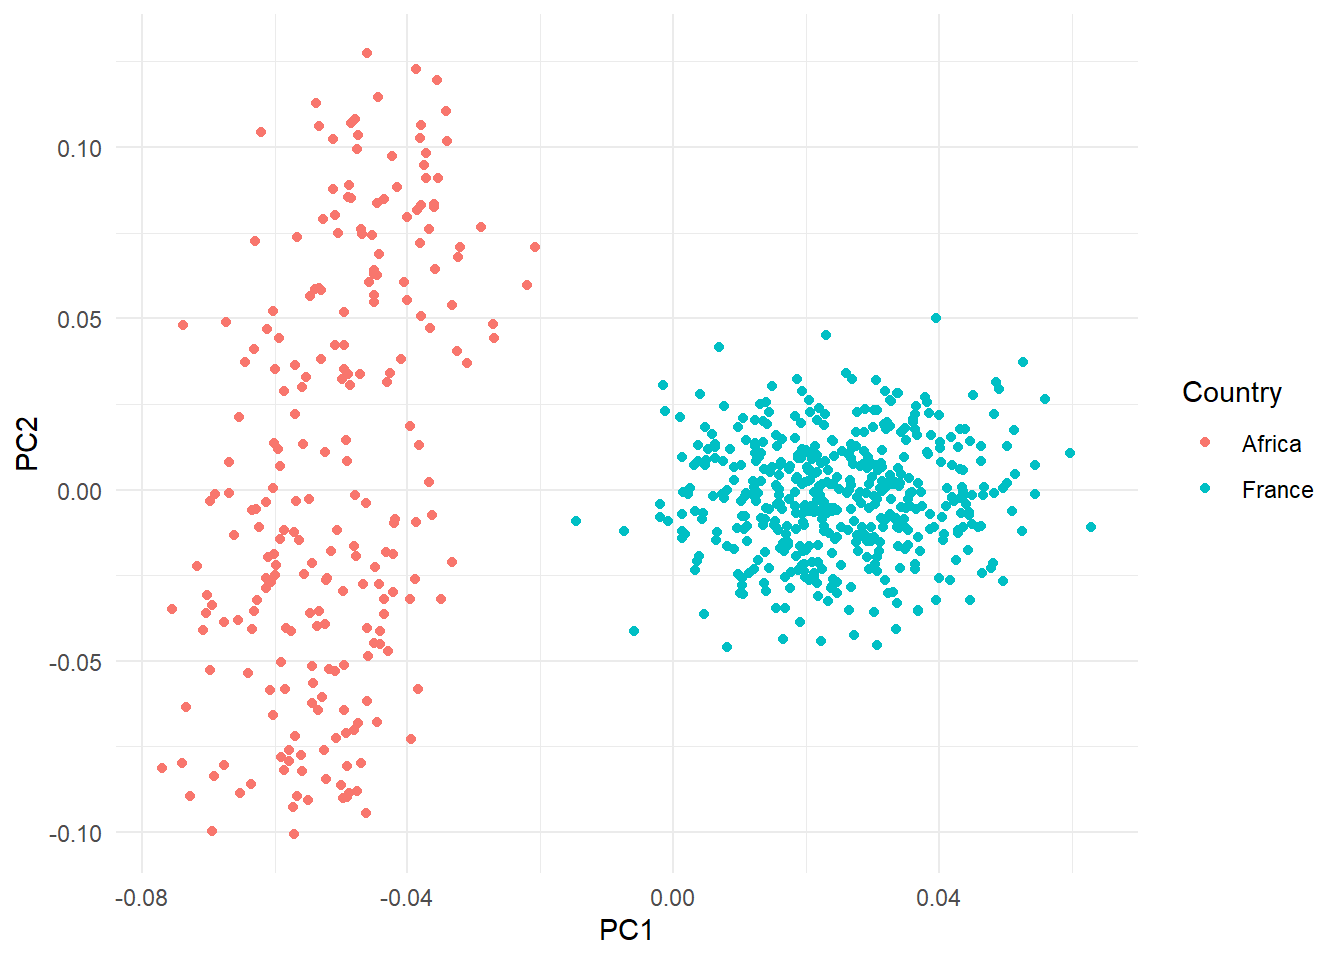
\includegraphics[width=0.75\linewidth,height=0.75\textheight]{PCAGenetics_files/figure-beamer/unnamed-chunk-4-1} \end{center}

\end{frame}

\begin{frame}{Bovines by breed}
\protect\hypertarget{bovines-by-breed}{}

\begin{itemize}
\tightlist
\item
  We also have each bovine's breed. We can see some separation with the
  first two principal components.
\end{itemize}

\begin{center}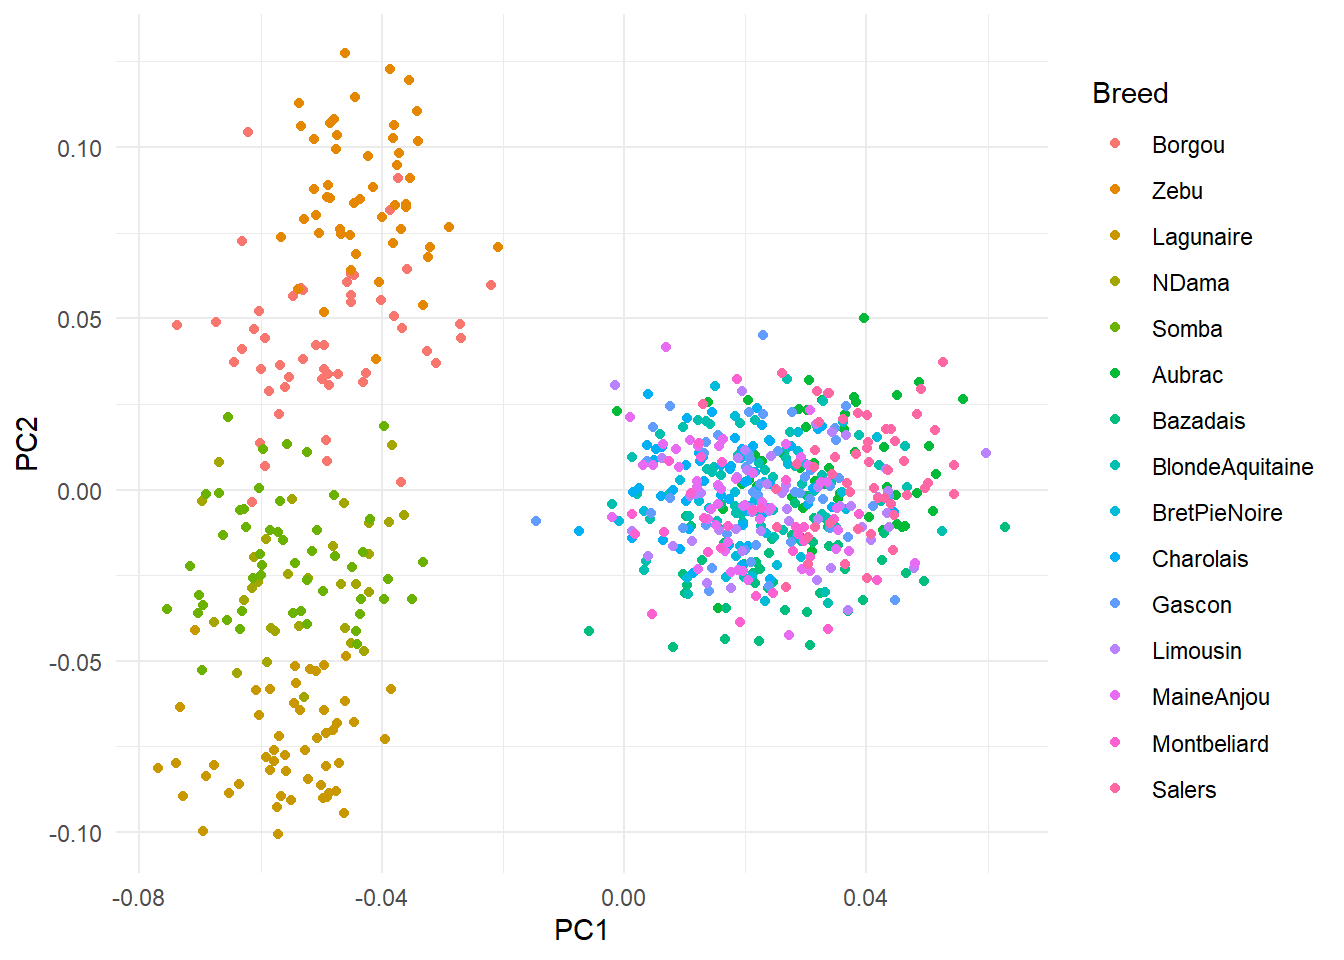
\includegraphics[width=0.75\linewidth,height=0.75\textheight]{PCAGenetics_files/figure-beamer/unnamed-chunk-5-1} \end{center}

\end{frame}

\end{document}
